\documentclass[doc,a4paper,floatsintext,draftfirst]{apa6}
\usepackage[]{graphicx}
\usepackage[]{color}

\usepackage{mwe,tikz}
\usepackage[percent]{overpic}


%% maxwidth is the original width if it is less than linewidth
%% otherwise use linewidth (to make sure the graphics do not exceed the margin)
\makeatletter
\def\maxwidth{ %
  \ifdim\Gin@nat@width>\linewidth
    \linewidth
  \else
    \Gin@nat@width
  \fi
}
\makeatother

\definecolor{fgcolor}{rgb}{0.345, 0.345, 0.345}
\newcommand{\hlnum}[1]{\textcolor[rgb]{0.686,0.059,0.569}{#1}}%
\newcommand{\hlstr}[1]{\textcolor[rgb]{0.192,0.494,0.8}{#1}}%
\newcommand{\hlcom}[1]{\textcolor[rgb]{0.678,0.584,0.686}{\textit{#1}}}%
\newcommand{\hlopt}[1]{\textcolor[rgb]{0,0,0}{#1}}%
\newcommand{\hlstd}[1]{\textcolor[rgb]{0.345,0.345,0.345}{#1}}%
\newcommand{\hlkwa}[1]{\textcolor[rgb]{0.161,0.373,0.58}{\textbf{#1}}}%
\newcommand{\hlkwb}[1]{\textcolor[rgb]{0.69,0.353,0.396}{#1}}%
\newcommand{\hlkwc}[1]{\textcolor[rgb]{0.333,0.667,0.333}{#1}}%
\newcommand{\hlkwd}[1]{\textcolor[rgb]{0.737,0.353,0.396}{\textbf{#1}}}%

\usepackage{framed}
\makeatletter
\newenvironment{kframe}{%
 \def\at@end@of@kframe{}%
 \ifinner\ifhmode%
  \def\at@end@of@kframe{\end{minipage}}%
  \begin{minipage}{\columnwidth}%
 \fi\fi%
 \def\FrameCommand##1{\hskip\@totalleftmargin \hskip-\fboxsep
 \colorbox{shadecolor}{##1}\hskip-\fboxsep
     % There is no \\@totalrightmargin, so:
     \hskip-\linewidth \hskip-\@totalleftmargin \hskip\columnwidth}%
 \MakeFramed {\advance\hsize-\width
   \@totalleftmargin\z@ \linewidth\hsize
   \@setminipage}}%
 {\par\unskip\endMakeFramed%
 \at@end@of@kframe}
\makeatother

\definecolor{shadecolor}{rgb}{.97, .97, .97}
\definecolor{messagecolor}{rgb}{0, 0, 0}
\definecolor{warningcolor}{rgb}{1, 0, 1}
\definecolor{errorcolor}{rgb}{1, 0, 0}
\newenvironment{knitrout}{}{} % an empty environment to be redefined in TeX

\usepackage{alltt}

\def\citeapos#1{\citeauthor{#1}'s (\citeyear{#1})}
\def\calH{{\cal H}}
\def\bfy{{\mathbf y}}
\def\bftheta{{\boldsymbol\theta}}


\usepackage{epigraph}
\usepackage{graphicx}
\usepackage{amsfonts}
\usepackage{amsbsy}
%\usepackage{setspace}
%\usepackage{pdfcomment}
%\usepackage{xspace}
\usepackage{color,amsmath,amssymb}
%\usepackage{framed}
\usepackage{enumerate}
\usepackage[caption=false]{subfig}

\usepackage[american]{babel}
\usepackage{csquotes}
\usepackage[style=apa,natbib=true,backend=biber]{biblatex}
%\usepackage[longnamesfirst]{natbib}
\DeclareLanguageMapping{american}{american-apa}

\usepackage{hyperref}


\usepackage[T1]{fontenc}
\usepackage[sc]{mathpazo}
\linespread{1.05}         % Palatino needs more leading (space between lines)

\bibliography{bibfile}
%\AtEveryBibitem{\clearfield{url}} 

\abstract{Low power in experimental psychology is an oft-discussed problem. We show in the context of the Replicability Project: Psychology (Open Science Collaboration, 2015) that sample sizes are so small in psychology that often one cannot detect even large differences between studies. High-powered replications cannot answer this problem, because the power to find differences in results from a previous study is limited by the sample size in the original study. This is not simply a problem with replications; cumulative science, which critically depends on assessing differences between results published in the literature, is practically impossible with typical sample sizes in experimental psychology. We diagnose misconceptions about power and suggest a solution to increase the resolution of published results.}


\shorttitle{Unfalsifiable psychology}

\leftheader{Morey and Lakens}

\twoauthors{Richard D. Morey}{Dani\"{e}l Lakens}

\title{Why most of psychology is statistically unfalsifiable}

\twoaffiliations{Cardiff University}{Eindhoven University of Technology}


%\theoremstyle{plain}
\newtheorem{theorem}{Theorem}
\newtheorem{proposition}{Proposition}
\newtheorem{lemma}{Lemma}
%\newtheorem*{corollary}{Corollary}

%\theoremstyle{definition}
\newtheorem{definition}{Definition}
\newtheorem{myth}{Fallacy}
\newtheorem{conjecture}{Conjecture}
%\newtheorem*{example}{Example}
\newtheorem{algorithm}{Algorithm}

%\theoremstyle{remark}
%\newtheorem*{remark}{Remark}
%\newtheorem*{note}{Note}
\newtheorem{case}{Case}

\setlength{\epigraphwidth}{5in}
\renewcommand{\epigraphflush}{center}
\renewcommand{\sourceflush}{flushleft}

\authornote{Address correspondence to Richard D. Morey (\href{mailto:richarddmorey@gmail.com}{richarddmorey@gmail.com}). All code and the source for this document are available at \url{https://github.com/richarddmorey/psychology_resolution}. Draft date: \today.}
\IfFileExists{upquote.sty}{\usepackage{upquote}}{}
\begin{document}

\maketitle

\setlength{\epigraphwidth}{\columnwidth}
\epigraph{``Obviously, an experiment designed [with low power] is not worth performing. Unfortunately, this particular point escaped the attention of a large number of authors of statistical texts...As a result, important experiments are often performed with the possibility of very frequent most regrettable errors.''}{\par\raggedleft\textup{Jerzy Neyman} (1977)}

\nocite{Neyman:1977}

Power is a crucial, often but poorly understood, statistical concept. Informally, power is often conceived of as a prospective assessment of the informativeness of a research design. More formally, it describes the ability of a statistical test to distinguish between values of a parameter of interest in a population. Tests that have low probability to distinguish between small and large effect sizes are of little use, and researchers are finally coming to terms with the fact that low-powered tests are a common problem. 

Lately, the robustness of the psychological literature has been tested by means of replication studies. If a well-designed experiment does not detect the presence of an effect, we have to ask ourselves why this has happened. One possibility is that the effect is highly context-dependent, and the right conditions were not met in the replication study. Having a discussion about potential causes of differences between an original and replication study presupposes that we can, in fact, determine whether two experimental outcomes are statistically different. When we look beyond the interpretation of replication studies, we see that cumulative science requires that we can detect differences between experiments that are not replications. In many fields, progress rests on controlled iterative changes to a research design, where differences or similarities between studies are used to test and develop theories. Many theoretical discussions in the literature hinge on our ability to identify such patterns of similarities and differences across studies. However, we cannot {\em explain} a difference before we have statistical evidence for the presence of a difference. Therefore, having sufficient statistical power to draw informative inferences about differences or similarities between two studies, such as an original and a replication study or two studies testing similar or different theoretical predictions, is essential in scientific research. If our goal is theoretical scientific progress, there is little point in performing experiments whose results cannot be compared to other studies in the literature.

Discussion sections in scientific papers often contain theoretical explanations of why one experiment showed an effect, but another did not. For example, Strack, Martin, and Stepper (1988) instructed participants to hold a pen in one's mouth in such a way that it activated muscles typically associated with smiling. In Study 1, this manipulation influenced funniness ratings. In Study 2, funniness ratings were unaffected, but amusement ratings differed between conditions. This was taken to suggest that ``subjects' ratings may often be a composite of both cognitive and affective factors, unless subjects are induced to distinguish between them'' (p. 775). Reviewers will often demand such discussions: What about {\em this other} paper? How do you reconcile the differences between {\em your} finding and {\em my} previous finding? The intuitive idea is that we can have  theoretical progress in psychology by examining the similarities and differences between experimental outcomes across studies. 

\nocite{Strack:etal:1988}

In this paper, we will show that even large differences between two similar experiments can often not be detected with high probability, due to the small sample sizes that have been typical in the psychological literature. We argue that as a consequence many of the findings in the psychological literature are in practice unfalsifiable. Due to the prevalence of small sample sizes, and the lack of any specification of the smallest effect size that would still support a theory, we conclude standard practice in psychology leads to studies that cannot be called into doubt by new statistical results. We will explore this general and fundamental problem in psychological science in detail by using the results from the Reproducibility Project: Psychology (RP:P; Open Science Collaboration, 2015) as a case-study. The RP:P offers a large number of similar pairs of experiments to illustrate our main points. However, our conclusions generalize to any attempt to learn from a pattern of effects across experiments. As such, the concerns we raise here about the unfalsifiability of psychological science calls into question whether a truly cumulative psychological science is currently possible. 

\nocite{OpenScienceCollaboration:2015}

To improve the falsifiability of psychological findings, we give practical recommendations to power future original research: sample sizes should be chosen such that a future, similarly-sized study would have a high chance of detecting a meaningfully-sized difference from the original study. If we desire scientific progress, experimental results should carry a risk of being falsified, and the minimal requirement for falsification is that two sets of findings can be demonstrated to differ statistically. 

\section{Power}

Suppose we wish to know whether personality is related to response times when categorizing simple stimuli. Moeller, Robinson, and Zabelina (2008) presented either the letter `p' or `q' on a horizontal or vertical axis, and asked participants to determine which letter was presented. They report that higher self-reported dominance on a personality scale was correlated with faster response times (measured as lower residual scores) on the vertical axis. The authors interpret this correlation as support for the idea that ``personality-related dominance...can be usefully understood in terms of vertical metaphoric processes'' (p. 359). Based on a sample of 53 participants they reported a correlation of $r=-0.31$ ($p=0.024$, CI$_{95\%}$: [-0.54, -0.04]). A replication attempt with 72 participants (OSC, 2015) obtained a correlation of $r=0.034$ ($p=0.777$, CI$_{95\%}$: [-0.2, 0.27]). We will use both the original and the replication results to illustrate power concepts.

\nocite{Moeller:etal:2008}

Often, hypothesis tests are used to test whether an true effect differs from~0, but we can test whether the true effect differs from any particular value. Suppose that we wish to test the hypothesis that the true correlation in the population, $\rho$, is 0.1, and we collect $n=53$ participants, as Moeller et al. did. Figure~\ref{fig:powexp1} shows (top) shows the distribution of the test statistic $Z$, Fisher's $z$ transformation\footnote{Fisher's $z$ transformation is an often-used transformation of the correlation coefficient that makes its sampling distribution approximately normal. Details can be found in the Appendix.} of the observed correlation $r$, under the hypothesis that $\rho=0.1$. The observed $Z$ value in the experiment, $z(-.31)=-.32$, is shown as a vertical gray line. If we wished to test the one-sided hypothesis that the true correlation is equal to or larger than 0.1, we see that the observed negative $Z$ value is quite extreme and surprising, assuming $\rho\geq0.1$. If $\rho\geq0.1$, the probability of obtaining a more extreme $Z$ value would be less than $p=.0015$. 

\begin{figure}
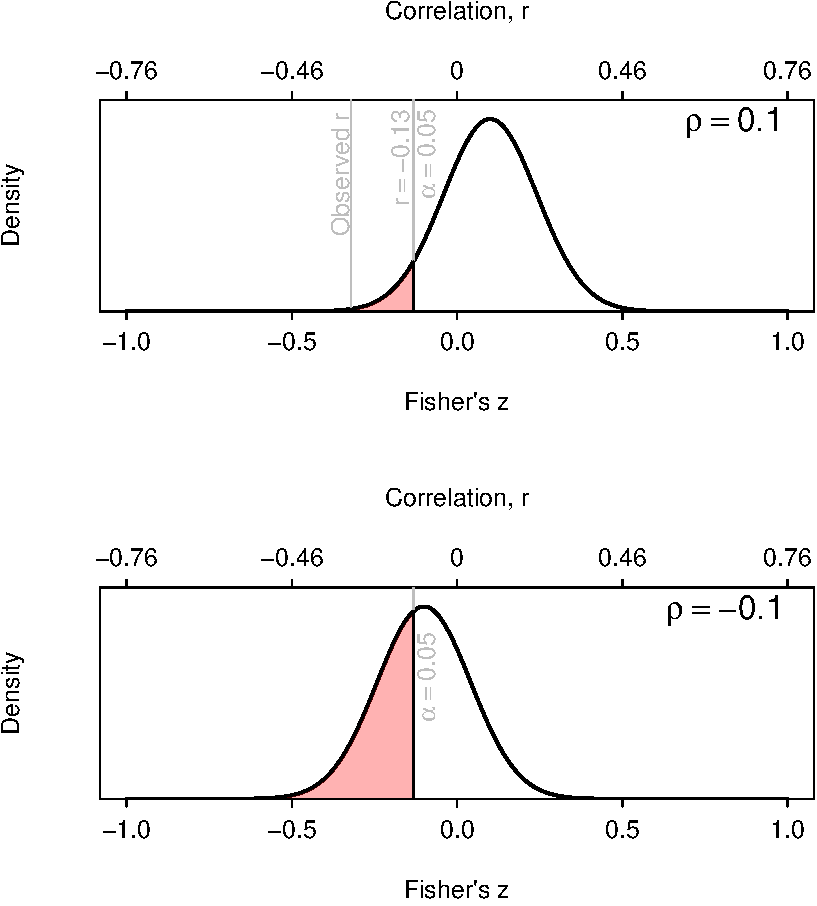
\includegraphics[width=\maxwidth]{figure/powexp-1} \caption{Building a test for $\rho\geq.1$. Top: If $\rho\geq.1$ then we would only rarely (less than 5\% of the time) find a correlation as low as -.13. (red shaded region). Under the hypothesis that $\rho=.1$, the observed $r$ is more extreme than would be expected 99.9\% of the time. Bottom: If $\rho=-.1$, we would find a correlation as low as $r=-.13$ just more than 41\% of the time (red shaded region).}\label{fig:powexp1}
\end{figure}

To construct a significance test with a desired error rate, we could choose a value of $Z<-.13$ (also $r<-.13$) as a critical value to reject our hypothesis that $\rho\geq0.1$, which would mean we do not incorrectly reject the null hypothesis more than $\alpha=5\%$ (the Type~I error rate) of the time, assuming $\rho\geq0.1$.

Whether this significance test is a good test or not depends not only on how often we incorrectly reject the null hypothesis when $\rho\geq0.1$, but also on the ability of the test to detect effects of interest smaller than $\rho=0.1$.  Assume that the effect in the population were actually $\rho=-.1$. Figure~\ref{fig:powexp1}(bottom) shows the distribution of $Z$ when $\rho=-.1$. If we adopt the criterion $Z<-.13$ for rejecting the hypothesis $\rho\geq0.1$ when in the population $\rho=-.1$, we would correctly reject $\rho\geq0.1$ with probability 0.41. That is, the {\em power} of the test at $\rho=-.1$ is 41\%.

\begin{figure}
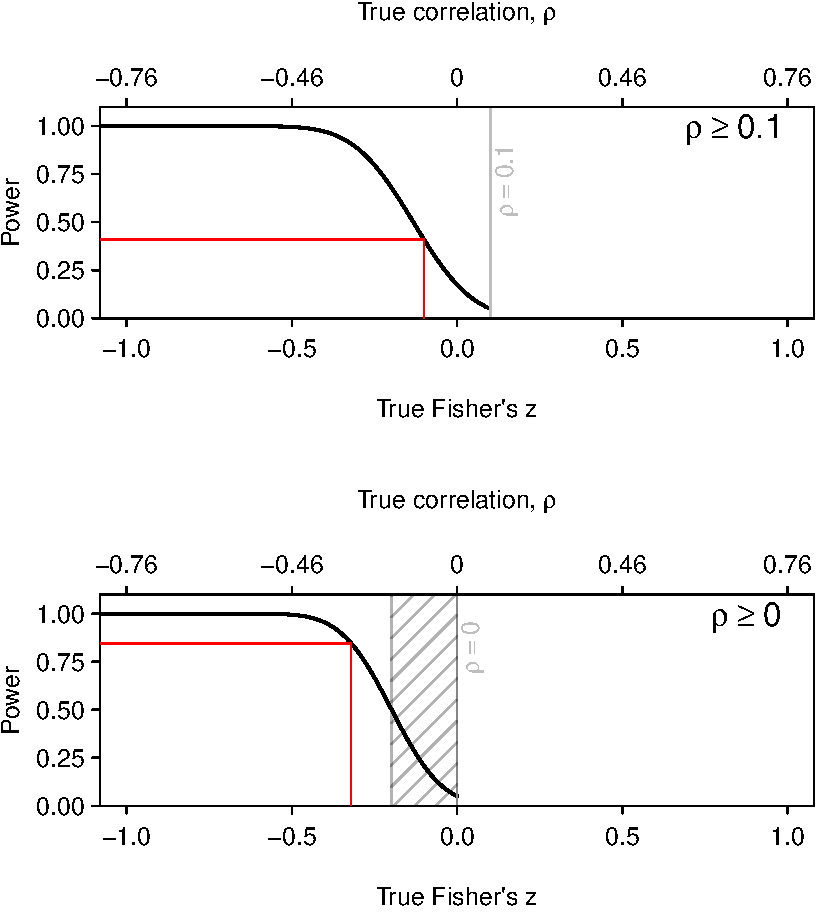
\includegraphics[width=\maxwidth]{figure/powexp2-1} \caption{Top: Power function for the test of $\rho\geq0.1$. The line segments correspond to the power for the alternative in Figure~\ref{fig:powexp1}, bottom. Bottom: Power curve for the OSC replication. The line segments correspond to the power assuming that $\rho$ equals the $r$ obtained by Moeller et al., the original authors. The shaded region indicates alternatives which have a power of less than 0.5.}\label{fig:powexp2}
\end{figure}

Although researchers often talk about ``the'' power of a test, and indicate the power of a test by a single value (e.g., 90\% power), a test has power to all hypothetically possible true values of the effect size. Therefore, it is important to think of statistical power as a curve of values such as that shown in Figure~\ref{fig:powexp2} (top). The figure shows the power of the test to reject the hypothesis that $\rho\geq0.1$ for all true values $\rho$ that are inconsistent with that hypothesis. For values of $\rho$ just below 0.1, the power is near 5\%. For values below $\rho=-0.5$, the test has very high statistical power and is almost sure to reject the null hypothesis of $\rho<0.1$. 

A key aspect of designing an informative experiment is choosing a sample size so that a test will be sufficiently powered for interesting values of the parameter. Sample size selection depends on a number of considerations, but when resources are not a major problem, or when it is essential that results from a study are informative, sample size should be chosen such that the test has high power to detect the effect sizes we would not want to miss (Senn, 2007). 

\nocite{Senn:2007}

It is useful to think of a statistical test as a smoke alarm; if we buy a smoke alarm, we would like to ensure that it would not sound too often if there is no smoke. If it would often sound when there is no smoke, we would probably (rightly) begin to ignore the alarm. On the other hand, if the alarm would {\em not} sound if there was a dangerous amount of smoke, then the alarm would not be useful. The alarm should be sensitive enough to detect concentrations of smoke that we regard as important. Finally, the alarm should not be overly-sensitive to unimportant concentrations of smoke (e.g., when blowing out a candle). If an alarm is too sensitive, we might increase the threshold for sounding. In a significance test this is analogous to reducing $\alpha$.

\section{Power and the Reproducibility Project: Psychology}

In the Reproducibility Project: Psychology (RP:P), the Open Science Collaboration (OSC; 2015) replicated 100 experiments in the psychological literature with the aim of assessing an initial estimate of how replicable psychological studies are. The OSC used a number criteria for success, including agreement in statistical significance and subjective ratings. Under one criterion --- agreement in statistical significance across the original and replications --- only 36\% of the studies replicated the original results. 

This dichotomous interpretation of replication success is of limited interest, since the replication studies only had high statistical power if we assume that the effect sizes reported in the original study were the {\em the smallest effect sizes of interest}. In this section we take a novel approach to assessing the {\em design} of the RP:P by use of a power analysis: If original and replication studies had very different underlying effect sizes, would the OSC have been able to detect these large differences in individual studies? We will analyze a subset of 73 of the study pairs in the RP:P.\footnote{These studies were chosen by restricting the set 92 studies selected by Patil, Peng, and Leek (2016) to those studies with effect sizes that had a single numerator degree of freedom.} The conclusions of our analysis echo those of \citet{Etz:Vandekerckhove:2016} in finding that many of the replication attempts were simply not informative. The root cause of this lack of informativeness is small sample sizes in original and replication studies. As we will show, these small sample sizes represent a serious problem for cumulative science.

\nocite{Patil:etal:2016}

The difference between the original study and the replication study can be quantified by the difference between their Fisher's $z$-transformed correlations, which we denote $d = z(r_{orig}) - z(r_{rep})$. The statistic $d$ is a measure of the disagreement between results of the original and the replication. For each of the 73 studies the difference between studies is shown in Figure~\ref{fig:resid1} as a function of the $r$ observed in the original and replication study (with all original correlations made positive for comparison). Because the difference is on the Fisher's $z$ scale (see appendix), it can be somewhat difficult to translate back into the correlation units with which most people are familiar. Figure~\ref{fig:zexp1}B shows the difference in $z$ units that corresponds to pairs of original and replication correlations. For instance, if a correlation of $r=0$ was found in the original and the replication found a correlation of $r=.5$, this would correspond to a difference in $z$ units of $d=-.55$. 


\begin{figure*}[ht]
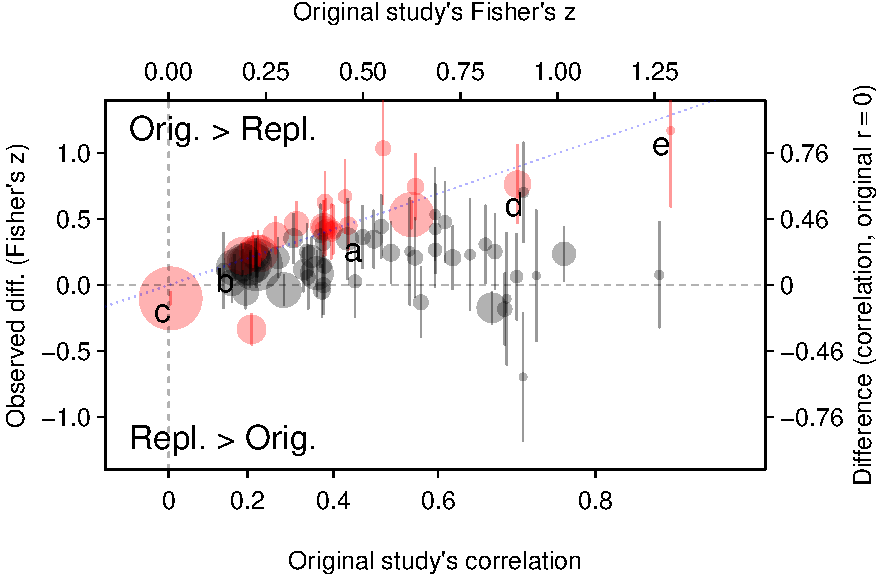
\includegraphics[width=\maxwidth]{figure/resid1-1} \caption{Original minus replication correlation (in Fisher's $z$ units) as a function of the original study's correlation for 73 of the 92 replication attempts selected by \citet{Patil:etal:2016}. Red points denote those attempts for which the replication and original were significantly different, $p<0.05$ (this corresponds to the 95\% prediction interval excluding the replication correlation). Error bars are standard errors; points on the diagonal line have a replication $r_{rep}=0$. The size of the points is proportional to the sample size in the original study. Letters to the lower-right of five points indicate the studies highlighted in Table~\ref{tab:studies}. An interactive version of this figure is available at \protect\url{https://richarddmorey.shinyapps.io/RPP_results/}.}\label{fig:resid1}
\end{figure*}

% latex table generated in R 3.2.2 by xtable 1.8-2 package
% Tue Aug  2 17:42:10 2016
\begin{table*}[ht]
\centering
\begin{tabular}{rlrrrrr}
  \hline
 & Orig. N & Repl. N & Orig. r & Repl. r & Deviation (Fisher's z) & Deviation SE (Fisher's z) \\ 
  \hline
{\em a} & 32 &   48 & 0.461 & 0.135 & 0.363 & 0.235 \\ 
 {\em b} & 186 &  280 & 0.167 & 0.037 & 0.132 & 0.096 \\ 
 {\em c} & 564 & 3597 & 0.005 & 0.106 & -0.102 & 0.045 \\ 
 {\em d} & 14 &   19 & 0.723 & 0.208 & 0.702 & 0.377 \\ 
 {\em e} & 8 &    8 & 0.860 & 0.120 & 1.171 & 0.577 \\ 
   \hline
\end{tabular}
\caption{Five studies from the RP:P that will be used for demonstration. See Figures~\ref{fig:resid1}, \ref{fig:pv_curve}, and \ref{fig:pv_curve2}.} 
\label{tab:studies}
\end{table*}

One way of assessing the similarity between the original and the replication studies in the RP:P is the $z$ score produced by dividing the difference $d$ between the two effect sizes by its standard error:
\[
z_d = \frac{d}{s_d}
\]
where the standard error $s_d$ is
\[
s_d = \sqrt{\frac{1}{n_{orig}-3} + \frac{1}{n_{rep}-3}}.
\]
Under the null hypothesis that the two studies have the same effect size, the $z_d$ scores will have a standard normal distribution. The standardized difference $z_d$ can be used as a test statistic for a test of no difference between the original and replication experiments. The standard error $s_d$ is the standard deviation of difference $d$ around its true value; when $s_d$ is large, estimates of the difference between the effect sizes will be highly variable. In this case the standard error can be used as a measure of uncertainty about the difference in the effect sizes. One important thing to note is that the standard error depends on both sample sizes equally; no matter how large $n_{rep}$ becomes, the uncertainty can never be reduced beyond what is allowed by the sample size $n_{orig}$ of the original study. We will see how this limitation becomes problematic when we try to answer questions about differences between studies in psychology, where sample sizes in original studies are often very small.

Figure~\ref{fig:power1} (top) shows the empirical cumulative density function of the $z_d$ scores, and the corresponding two-tailed $p$~values (top axis) for the test of no difference using the $z_d$ score. This empirical cumulative density function is a way of visualizing the proportion of $z_d$ scores that are lower than a particular value. We know, for instance, that we would expect half of $z_d$ scores to be less than 0 if there were truly no difference. What we find, however, is that only about 10\% of the $z_d$ scores for original and replication studies in the RP:P are less than 0. Overall, these $z$ scores deviate substantially from the distribution we would expect if there were no difference between replication studies and original studies (red dashed line). The theoretical $z$ distribution under the assumption of no difference between original and replication studies has a median of 0; the observed $z$ scores in the RP:P have a median of ~1.4. Moreover, roughly 30\% of the pairs of studies show differences that would be flagged as ``significant'' at $\alpha=0.05$.\footnote{This is different from the 25\% reported by Patil et al (2016). As we explain later, we removed several pairs of studies from their analysis that had been inappropriately included.} In the aggregate, these results appear to indicate that something is amiss; the replication studies have effect sizes that are, on average, substantially lower than the original studies (as discussed in OSC, 2015).


The RP:P was meant to assess the reliability of studies in the psychological literature. Setting aside issues about the faithfulness of the replications and assuming the best possible scenario in which the replication studies can be said to be testing the same hypotheses as the original studies, if there {\em were}, in fact, a difference between the effect size in an original and a replication study, the RP:P should have a high probability of detecting it. Key to this is having high power.

Unfortunately, despite the fact that statisticians have warned against using effect size estimates from small samples in power analyses (e.g., Leon, Lore, and Kraemer, 2011), sample sizes in the RP:P studies were only powered to detect effects as large as the one observed in the original experiment. This method of performing a power analysis will yield under-powered tests whenever publication bias inflates effect sizes in the literature. The consequence is that although the studies had a high probability to reject the null hypothesis {\em if} the effect size estimates in the original study were the true effect sizes --- a dubious assumption, to say the least --- the replication studies had poor power to detect even large differences between the original study and the replication study. Figure~\ref{fig:power1} (bottom) shows the power curves for all the 73 replication studies included in our analysis for an $\alpha=0.05$ test of the difference.

\nocite{Leon:etal:2011}

The median power to detect a deviation of 0.3 Fisher's $z$ units from the original is only .29. One-quarter of studies had a power of less than .19 to detect the same difference. Only 11\% of studies had a power of above 0.8 to detect a deviation of 0.3 $z$ units. To put this difference of .3 $z$ units in context, see Figure~\ref{fig:zexp1}B. If the true correlation in the original were $\rho=0$, then a true difference of .3 Fisher's $z$ units would mean that the replication had a true correlation of .3.  If the true correlation in the original were $\rho=.5$, then a true difference of .3 Fisher's $z$ units would mean that the replication had a true correlation of .24 or .70. Because most studies had correlations around 0, one would not be far off assuming that a difference of 0.3 Fisher's $z$ units corresponds to a difference of 0.3 correlation units. In terms of Cohen's descriptors, this represents the difference between having a ``medium'' effect size, and having none at all.

\nocite{Cohen:1988}

Not until the true difference is increased to about 0.79 (that is, if $r_{orig}=0$, then $r_{rep}=.66$) --- a {\em very} large deviation from the original --- do 75\% of studies have a power of 80\%. Except in the aggregate, the RP:P studies are not well-suited to test the robustness of the psychological literature, if this question is defined as whether the results of replications differ substantially from the original results.

\begin{figure}
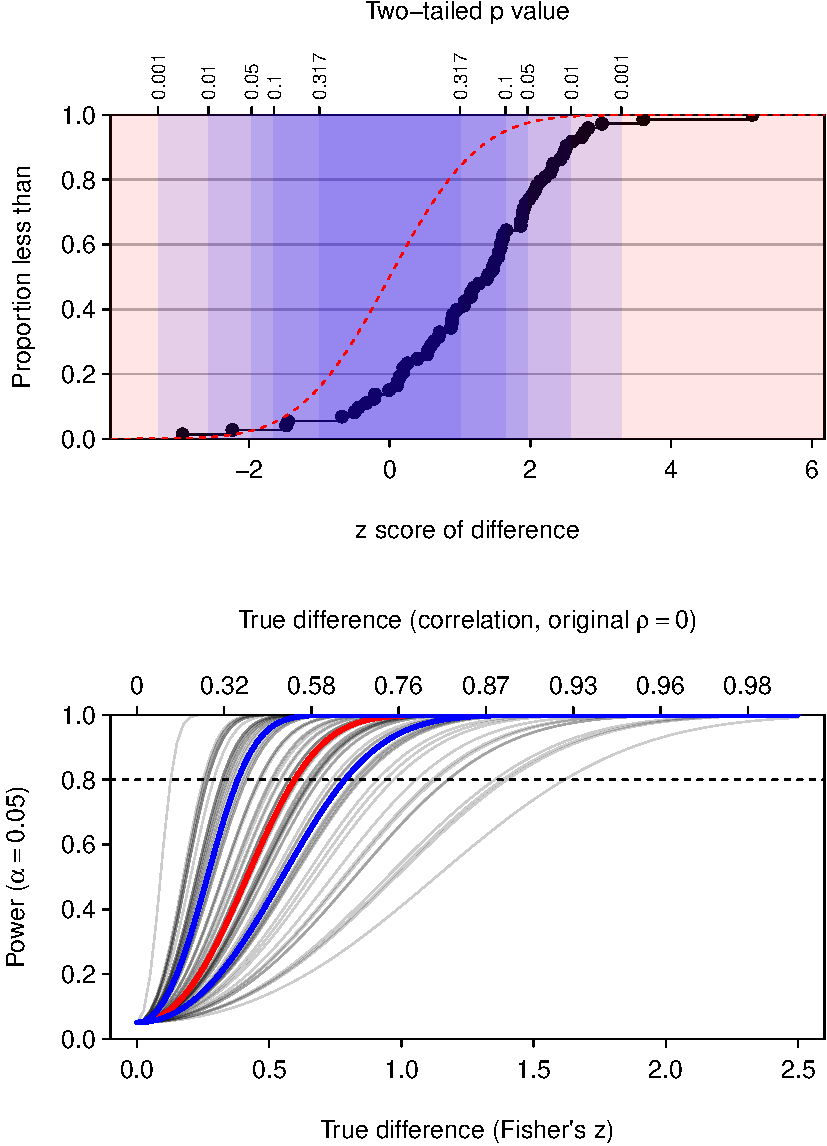
\includegraphics[width=.9\maxwidth]{figure/power1-1} \caption[Top]{Top: the empirical distribution function (ECDF) of the $z$ scores for the test that the original and replication correlations are the same. The red dashed curve represents the expected ECDF for true replications. Bottom: Power curves to detect specified deviations from equality, given the sample sizes in the original and replication attempts. Each gray curve is a replication attempt. The thick red curve shows the median power at that effect size, and the lower and upper thick blue curves show the first and third quartiles of the power, respectively. An interactive version of the bottom figure is available at \protect\url{https://richarddmorey.shinyapps.io/RPP_results/}.}\label{fig:power1}
\end{figure}

\subsection{Assessing the size of the differences}
The power analysis tells us that that, {\em a priori}, we should not expect to detect even large differences between the original studies and the replications based on the sample sizes of original and replication studies in the RP:P. This knowledge will be useful for future replication projects, but is not very useful when we want to know what conclusions we can draw from the 73 replication studies. So how can we enable researchers to design better studies in the future, that will enable cumulative science? Here, we calculate one-sided $p$~values to bound the sizes of the differences from the original studies.\footnote{These one-sided $p$~values are related to the frequentist logic of severity \citep{Mayo:Spanos:2006a}, equivalence testing (Schuirmann, 1987, Wellek, 2003), and that of confidence intervals (CIs); however we downplay this relationship because of the ease with which people fall into the so-called ``fallacy of acceptance'' (Mayo \& Spanos, 2006): that because a value is in a confidence interval, that value is plausible. The logic of tests also allows us to talk about the important concept of power. Finally, use of curves of $p$ values avoids us having to choose an arbitrary confidence coefficient, reducing the degree to which we encourage dichotomous thinking from confidence intervals.} 

\nocite{Wellek:2003,Schuirmann:1987}

Consider the top panel of Figure~\ref{fig:pv_curve}. The black density line represents the distribution of the difference between the original and replication correlations under the null hypothesis of no difference. The $p$ value for the test of no difference --- the probability of result as large as the one observed, assuming no difference --- in study {\em a} is represented by the gray shaded area under this distribution beyond the observed difference of .36. For this particular study the two-tailed $p=0.12$. 

Although it is, unfortunately, most common to examine only the $p$~value for the hypothesis of no difference, we can just as easily compute $p$ values that correspond to other hypotheses. Consider the red dashed density in Figure~\ref{fig:severity1} (top left); this represents the distribution of the observed difference if the true difference between the original and replication were .3 Fisher's $z$ units. Under the hypothesis that the true difference is .3 Fisher's $z$ units we would expect the values to be larger, on average, than if the difference were 0.

The red shaded region is the $p$~value for testing the hypothesis that the absolute value of the difference is {\em at least} 0.3. A low $p$ value for this test can be used to reject a true difference larger than 0.3: differences this {\em small} would be rare if the true difference were at least 0.3. For the study represented in the top panel, this $p$ value --- which we denote $p_{>.3}$ to differentiate it with the test of the null hypothesis --- is $p_{>.3}=0.6$. The high $p$~values in both these tests indicates the observed effect is not surprising enough to reject the hypothesis that the difference is zero, but also not surprising enough to reject the hypothesis that the absolute value of the difference is at least .3, at commonly-used $\alpha$ levels. 

A second study, study {\em b}, is represented in the lower panels of Figure~\ref{fig:pv_curve}. As for study {\em a}, the $p$~value testing the hypothesis of no difference is large at $p=0.17$, because the $z$ score for testing the sameness of the original and replication are similar between studies~{\em a} and~{\em b}. However, the test of the hypothesis that the absolute value of the difference is at least .3 turns out differently for study {\em b}: $p_{>.3}=0.04$ (red shaded region). The observed difference between the original and replication for study {\em b} is quite small relative to the sampling distribution of differences under the hypothesis that the true difference is .3, and hence, we would reject the hypothesis that the absolute value of the difference between the effect sizes in the original study and the replication study is greater than .3 at any $\alpha$ above .04.

These two replication attempts both led to non-significant differences between the original and replication correlations. A simple significance test of whether the difference is 0 does not differentiate them. The two studies are, however, very different. As Table~\ref{tab:studies} shows, the standard error of the difference for the first study is much larger, and Figure~\ref{fig:resid1} shows that the original and replication were much more similar in pair {\em b}. The original and replication in study {\em b} had sample sizes {\em six times larger} than those for study {\em a}. Our resolution for seeing differences between studies is better with higher sample sizes.


\begin{figure*}
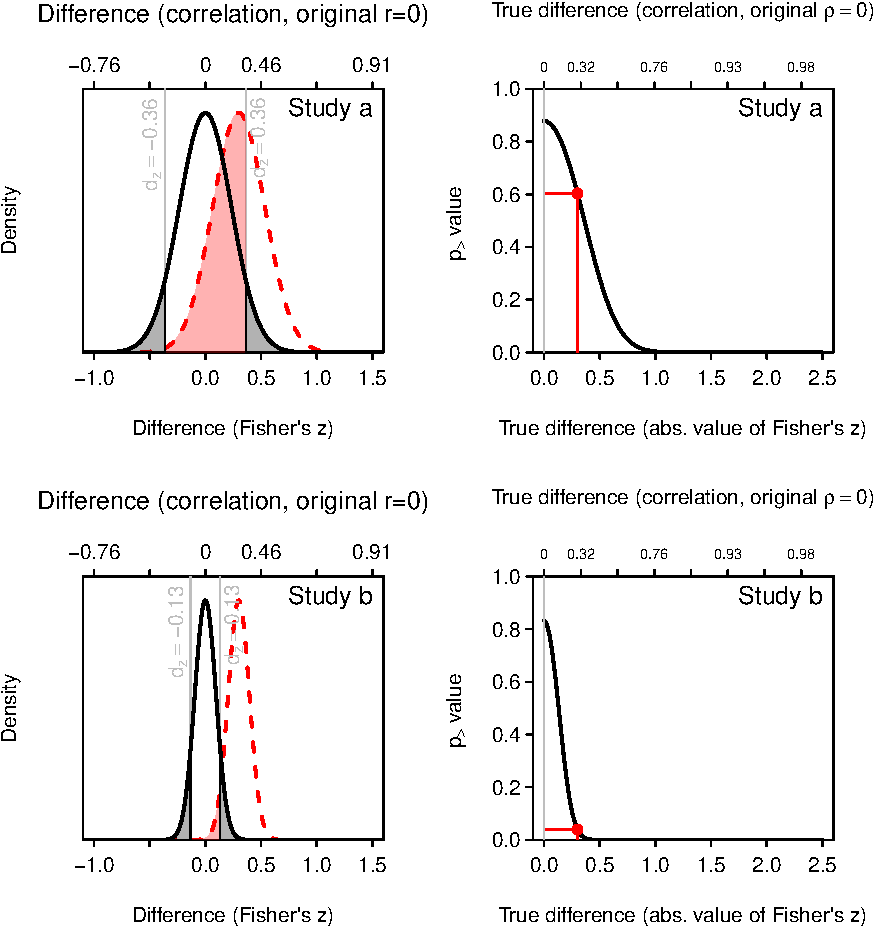
\includegraphics[width=.9\maxwidth]{figure/severity1-1} 
\vspace{.1in}
\caption[Sampling distributions of test statistic ]{Right column: Sampling distributions of the difference the original and replication correlations. The top and bottom panel represent two different replication attempts in the RP:P. Black distribution: Null distribution of no difference. Dashed (red) distribution: A true deviation in Fisher's $z$ units of 0.3. The gray shaded region represents the $p$ value testing no difference (studies~{\em a} and~{\em b}, $p=0.12$ and $p=0.17$, respectively); the red shaded region represents the $p_{>}$ value testing that the difference is at least than 0.3 (studies~{\em a} and~{\em b} $p_{>.3}=0.6$ and $p_{>.3}=0.04$, respectively). Left column: Curves of $p_{>}$ values as a function of deviation between original and replication study. An interactive version of this figure is available at \protect\url{https://richarddmorey.shinyapps.io/RPP_results/}.}\label{fig:pv_curve}
\end{figure*}

We are not limited to testing hypotheses such as those examining whether a difference is greater than 0.3; we can compute the $p_{>}$ values for ranges of differences. Figure~\ref{fig:pv_curve} (top, right) shows the $p_{>}$ values for study {\em a}, testing the every hypothesis of the form $\delta\geq \delta_0$, where $\delta$ is the true deviation and $\delta_0$ is a upper bound. The curve for study {\em a} in Figure~\ref{fig:pv_curve} (top right) is much more spread out than that for study {\em b} (bottom right), indicating that we can rule out much smaller differences in effect sizes in study {\em b} than in study {\em a}.

Figure~\ref{fig:pv_curve2} (top) shows the $p_{>}$ curve for every one of the 73 studies we analyzed. Replication studies in which the replication yielded a significant difference from the original are represented by dashed lines. Where a curve dips near the bottom, the test against that alternative has a low $p_{>}$ value; using the logic of the significance test we infer that the difference between the original and the replication study is {\em less than} the deviation on the $x$~axis. The important thing to note is that for most replication studies we cannot even infer that the difference is less than some very large deviation. From a perspective where we would like replication studies to yield at least somewhat similar effect sizes, this is difficult news. If we cannot infer that the difference between the original and replication study is less than, say, 0.5 Fisher's $z$ units, we can neither infer that the replication was ``successful'' nor that it ``failed''; the best we can say is that the data are not informative.

The bottom panel of Figure~\ref{fig:pv_curve2} shows the proportion of non-significant replication studies for which $p_{>}<0.05$, for all deviations. We choose a criterion of $p_{>}<0.05$ by convention and for demonstration. Only 20\% of non-significant studies can be inferred to have a difference of less than .3. Only about 60\% of these replication studies can be inferred to have a difference of less than 0.5, which represents a very large difference in true correlations. For 60\% of the RP:P pairs, we are unsure whether the difference is larger than the difference between a study with a ``large'' correlation and one no correlation (using Cohen's 1988 labels). 

\nocite{Cohen:1988}

\begin{figure}
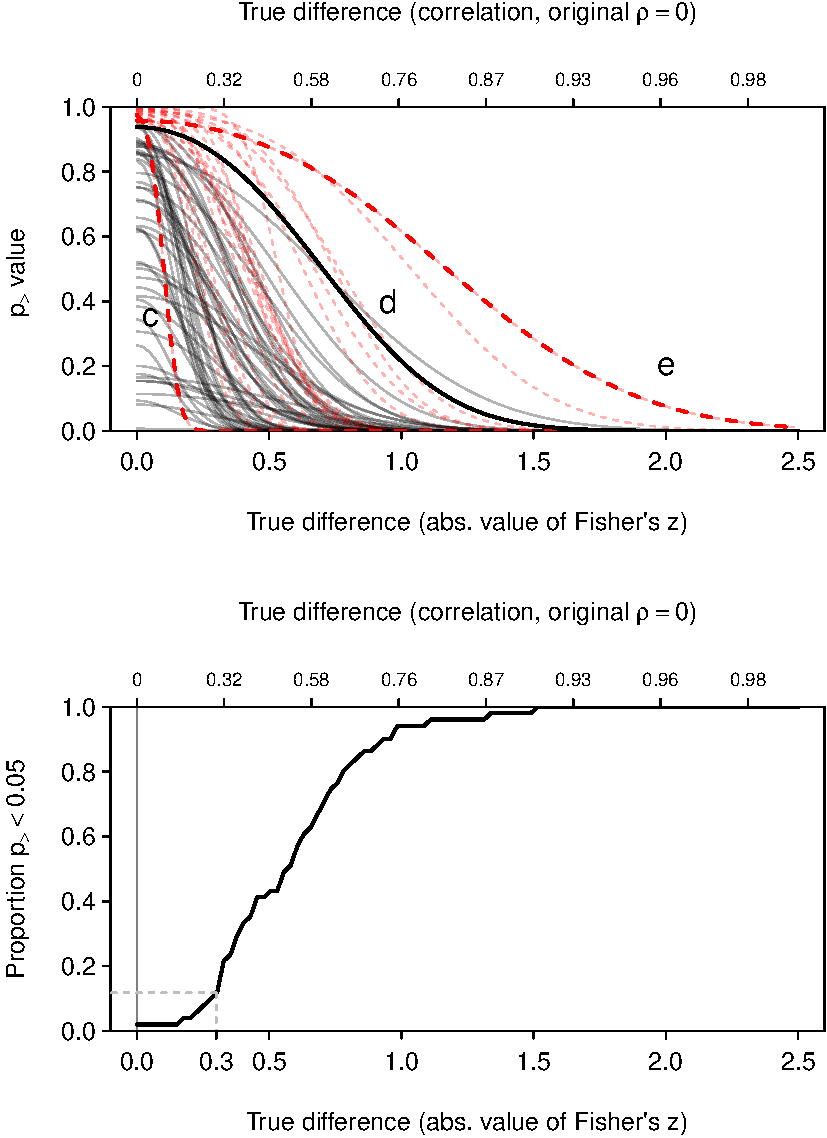
\includegraphics[width=.9\maxwidth]{figure/severity2-1} \caption[Top]{Top: $p_{>}$ values testing the hypothesis that the difference between the original and the replication study is smaller than the value on the $x$ axis. Solid lines represent replication attempts whose difference test is non-significant; dashed lines represent replication attempts whose difference test is significant. See text for an explanation of the thick black lines. Bottom: The proportion of $p_{>}$ values less than 0.05 for given deviations, for 51 the studies for which there was a non-significant difference between the original and the replication. An interactive version of the top figure is available at \protect\url{https://richarddmorey.shinyapps.io/RPP_results/}.}\label{fig:pv_curve2}
\end{figure}

\subsubsection{Low power and falsification}

In our opinion, one of the most important contributions of the RP:P was not that it showed that many findings in psychology did not replicate {\em per se}. Rather, it showed that many studies in psychology are practically not falsifiable. Consider one of the studies replicated in the RP:P that had a sample size of 9 participants (study {\em e} in Table~\ref{tab:studies}). Could a reasonably-sized replication study have any chance of detecting a large difference in effect size from the original? 

If we consider the standard error $s_d$ of the test of no difference between the original and replication studies, we note that it includes the sum of two terms: the variance of the effect size $Z_{orig}$ in the original study, $1/(n_{orig}-3)$, and the variance of the effect size $Z_{rep}$ in the original study, $1/(n_{rep}-3)$. When planning a typical study, we know that increasing the sample size will yield arbitrarily high power because the standard error of the parameter estimate approaches 0. However, when designing a replication study, increasing the sample size of the replication study does {\em not} yield arbitrarily high power to detect a difference with the original study: although $1/(n_{rep}-3)$ may approach 0, $s_d$ cannot, because it also depends on $n_{orig}$ which we cannot control. This means that the power to find a difference between the original and replication studies is always limited by the sample size of the original study. The power curve for the difference in effect sizes as $n_{rep}\rightarrow\infty$ will be the same as the power curve for the effect in the original study.\footnote{See the interactive demonstration at \url{https://richarddmorey.shinyapps.io/powerDiff/}.} Given this fact, original studies with small sample sizes are, in practice, unfalsifiable. 

Another way to understand this is through the CI on the difference between the original and the replication. Its width is affected by two sources of uncertainty: the uncertainty of the effect size in the original study and the variance of the parameter estimate in the replication study. One can reduce the second source of uncertainty to an arbitrarily small level by collecting a suitably large sample, but the uncertainty from the original will always remain, and hence the width of the interval on the difference can never be narrower than the CI on the original effect.


\begin{figure}

\subfloat{%
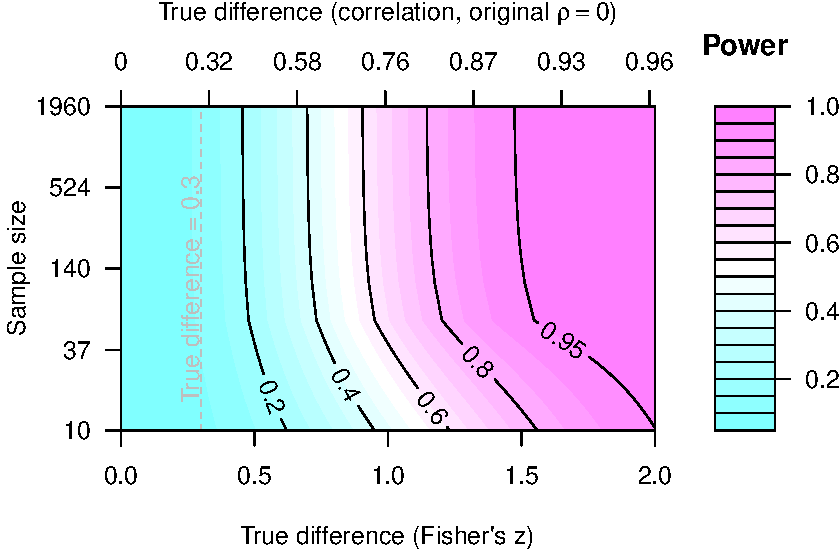
\includegraphics[width=.9\maxwidth]{figure/reppower1-1} 
}

%\vspace{-.2in}
\subfloat{%
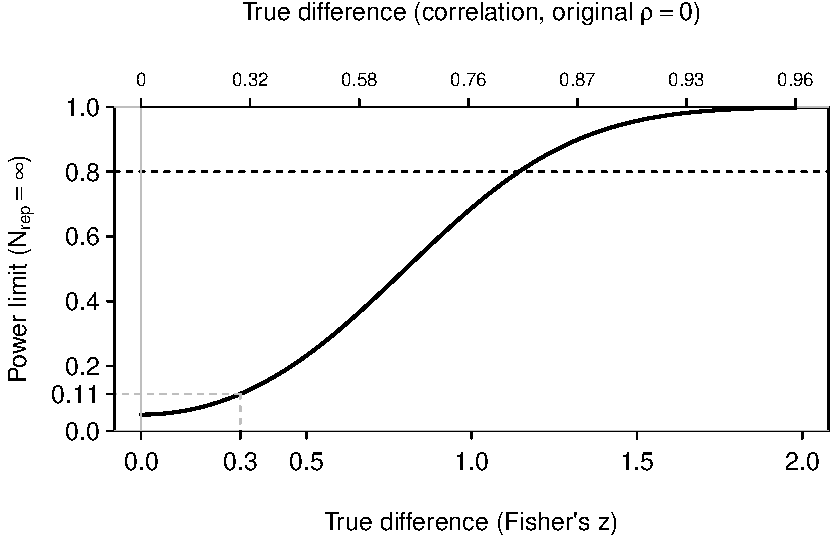
\includegraphics[width=.9\maxwidth]{figure/reppower2-1} 
}

\caption{Power to detect various deviations from equality of the original and replication studies, assuming $N_{orig}=9$. Top: Power as a function of the deviation and $n_{rep}$. Bottom: The limit (as $n_{rep}\rightarrow\infty$) on the power. An interactive application demonstrating powering to differences is available at \protect\url{https://richarddmorey.shinyapps.io/powerDiff/}.}
\label{fig:reppower}
\end{figure}


This limit on power from small original studies has dramatic consequences for the replication studies in the RP:P. Consider study {\em e} from Table~\ref{tab:studies}, which had an extremely small original sample size and very large observed effect size. The replication was powered by assuming the effect size found by the original study was the true effect, which led to abysmal power to detect differences between the two studies (as seen in Figure~\ref{fig:pv_curve2}). What if the replicators had chosen a larger sample size? Figure~\ref{fig:reppower} (top) shows how sample size in the replication study affects the power to detect differences between the original and replication studies. For a deviation of $0.3$ Fisher's $z$ units, the power cannot exceed 0.11, {\em regardless of how many participants would be run in a replication}. The sample size from the original study was simply too small. The bottom panel of Figure~\ref{fig:reppower} shows the limit of the power as $n_{rep}\rightarrow\infty$; that is, as we obtain an infinite number of participants in the replication. Even if the replication study had included an infinite number of participants, it would have had not have had a power of 0.8 to detect true differences as large as 1 Fisher's $z$ unit. To put this into perspective in correlation units, if the original study had a true correlation of $\rho=.76$, and the replication had a true correlation of $\rho=0$, {\em the replication would not have had 80\% power to detect this dramatic difference.}

The small size of the original studies makes it  practically impossible to reasonably argue that another study has yielded different results. If the RP:P shows that ``the replication rate in psychology is...statistically indistinguishable from 100\%'' --- as Gilbert et al (2016) argue --- it is only because studies are often so poorly powered that even large differences between studies cannot be detected. Many studies in psychology are in little danger of being falsified, because they make no risky predictions about what a replication should find --- neither statistically nor theoretically. For these studies, replication attempts are practically predetermined to be non-informative about potential differences between the original and the replication.

\nocite{Gilbert:etal:2016}

\section{How we got here: Power fallacies}
Poor understanding of power has long been a problem for users of significance tests. Neyman (1977), for instance, says that ``[u]nfortunately, [the problem of low powered tests] escaped the attention of a large number of authors of statistical texts. Yes, the concept of power is occasionally mentioned, but its treatment is somewhat `platonic'.'' Sedlmeier and Gigerenzer (1989) reviewed the entire 1984 volume of {\textit Journal of Abnormal Psychology} and ``found almost no concern with power expressed...'' Cohen (1992) laments that ``[i]t is not at all clear why researchers continue to ignore power analysis. The passive acceptance of this state of affairs by editors and reviewers is even more of a mystery.'' More recently, Fritz, Scherndl, and K\"{u}hberger (2012) reported that only on average, only about 3\% of articles reported a power analysis.

\nocite{Cohen:1992,Neyman:1977,Fritz:etal:2013,Sedlmeier:Gigerenzer:1989}

As we re-examine methods in psychology, one of the areas that has received attention is power (e.g., Button et al, 2013). However, the modern treatment of power is riddled with fallacies about power analysis. This has a unfortunate effect that although researchers may {\em believe} their studies are ``high-powered'' --- as the OSC believed --- they actually are not. We review four common power fallacies here.

\nocite{Button:etal:2013}

{\bf Misconception 1: Experiments have actual/observed/{\em post hoc} power.} We often speak loosely about ``low-powered'' studies. However, studies do not have power; only statistical tests have power. More correctly, {\em tests} have {\em power curves}. We can say that a test has low statistical power for an assumed effect size, but since the true effect size is unknown, and a range of effect sizes is often plausible and theoretically interesting, the statistical power of a test is indicated by a curve covering a range of effect sizes. When we casually talk about a ``low-powered study'',  what is typically meant is that the test of the focal hypothesis has a power {\em curve} that is low for interesting deviations from the null hypothesis. Importantly, power is a way of evaluating the quality of a statistical test that can be applied in situations where the true effect size is null, small, or very large. The power is the same in all these situations.


The use of casual language about studies having a specific power, such as in the RP:P where the ``average replication power'' is indicated as 92\%,  has led to the incorrect belief that the power of a test depends on the true value of the parameter. Since this true value is unknown, the power of a test depends not on what the effect size {\em is}, but rather on {\em all the hypothetical values it could be}. A sensitive smoke alarm is sensitive regardless of the actual amount of smoke in the room; it is sensitive when we know that {\em if} there were a dangerous amount of smoke in the room, the alarm would sound. Two identical fire alarms are equally sensitive despite one being in a smoke-filled home and the other not. Attempts to ``estimate'' the power of an experiment, or a field, are based on a misunderstanding of power and are uninformative and confusing (Goodman \& Berlin, 1994; Hoenig \& Heisey, 2001; O'Keefe, 2007).

\nocite{Hoenig:Heisey:2001,Goodman:Berlin:1994,OKeefe:2007}

This misunderstanding has likely been exacerbated by the way that power is taught in introductory methods courses. Figure~\ref{fig:powtab1} (top) shows a $2\times2$ table of the sort often presented in applied statistics texts. The ``state of nature'' is dichotomized into the null hypothesis and a single alternative against which there is a single level of power, $1-\beta$. This dichotomization encourages one to ask ``If the null hypothesis is not true, what single value might it be?'' and then inferring that it must be the ``true'' value in the study. The premise underlying the question is wrong. The alternative is a composite of many possibly interesting values, not a single value. The use of the $2\times2$ table has inadvertently caused misconceptions about power.

\begin{figure}
  \begin{overpic}[width=.8\maxwidth]{figure/powtab-1}
     \put(52,45){
\includegraphics[scale=.66]{figure/incorrect}}
     \put(50,5){
\includegraphics[scale=.075]{figure/ticks}}  
  \end{overpic}
%%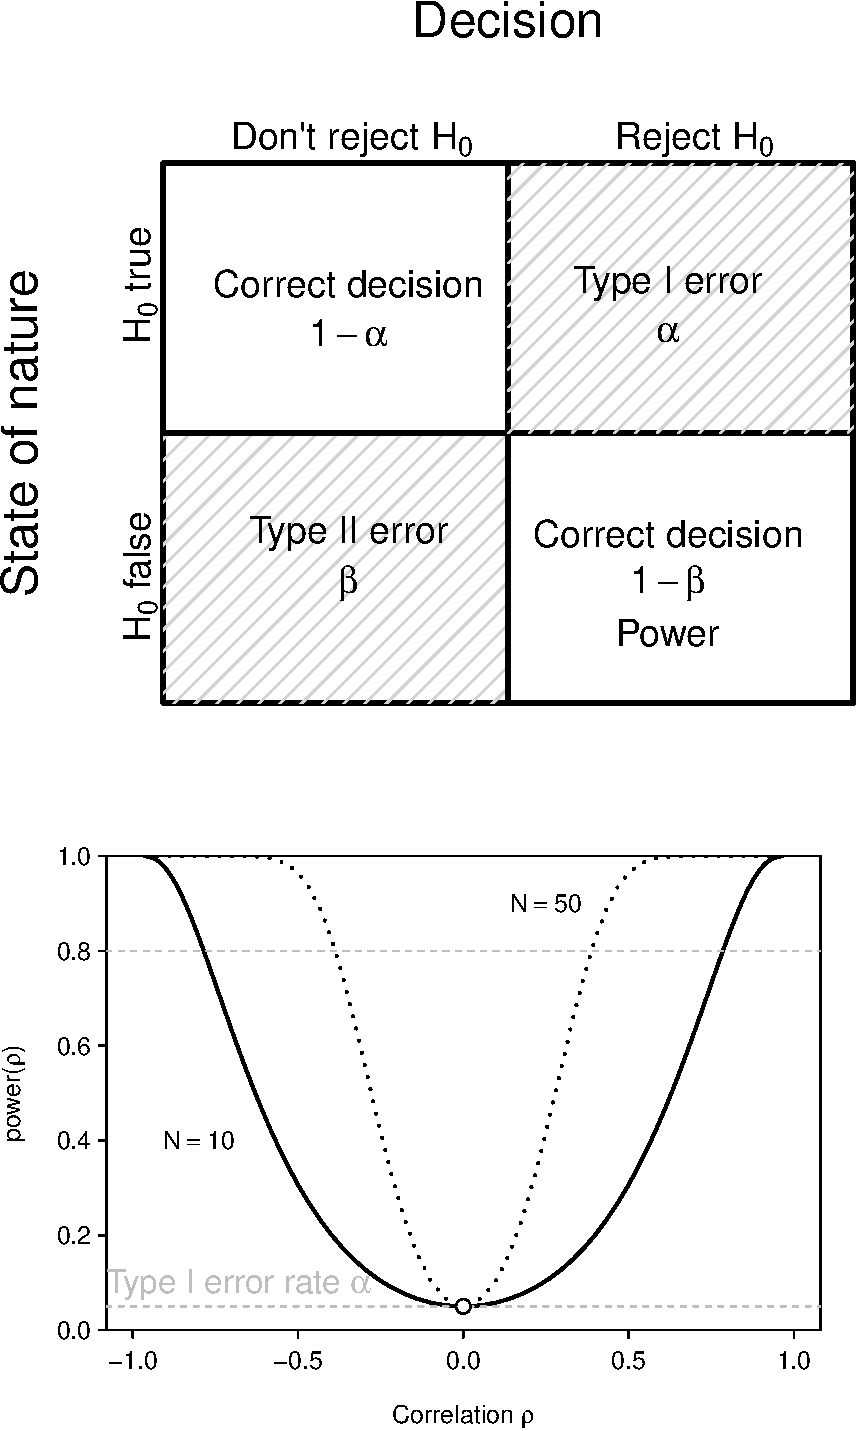
\includegraphics[width=\maxwidth]{figure/powtab-1} 
\caption{Two ways of describing power. Top: The typical way power is described in introductory textbooks. Bottom: The preferred way, as curves (one for n = 10 and one for n = 50), to emphasize the composite nature of the alternative and that power is a {\em function} of hypothetical effect sizes.}
\label{fig:powtab1}
\end{figure}

If we present power properly as a function, as in Figure~\ref{fig:powtab1} (bottom), then fallacies are easier to avoid. The test has power to all values of $\rho$, not just to a single ``true'' value. Whether a test is high-powered or not can be determined by assessing the height of the function at interesting values of $\rho$, for any given design, test, and sample size.

{\bf Misconception 2: Power is a conditional probability.}
One of the ways that power is often defined in introductory statistics texts is ``Power is the probability of rejecting $H_0$ given that $H_0$ is false.'' This is often incorrectly rendered in symbols as
\[
\mbox{Power} = Pr(p\leq 0.05\mid H_a)
\]
for an alternative hypothesis $H_a$; or, alternatively (but distinctly from above),
\[
\mbox{Power} = Pr(p\leq 0.05\mid \rho=\rho_1)
\]
where $\rho_1$ is any value of $\rho$ other than the null hypothesis. Both of these renderings are incorrect as a matter of frequentist statistics: neither $H_a$ nor $\rho$ is random, and hence neither would be conditioned upon.

The avoidance of the conditional stroke is not simply a frequentist ideological choice. Conditional probability must be defined in terms of a joint probability and marginal probability. By the definition of conditional probability,
\[
Pr(p\leq 0.05\mid \rho=\rho_1) = \frac{Pr(p\leq 0.05,\rho=\rho_1) }{Pr(\rho=\rho_1)}.
\]
The probability $Pr(\rho=\rho_1)$ in the denominator of the right-hand side must be either 0 or 1, depending on whether $\rho=\rho_1$ or not. But if the denominator is 0, then the probability --- which might be power or a Type~I error rate, incorrectly rendered --- would cease to exist for all but one, unknown value of $\rho$.\footnote{In Bayesian statistics, $Pr(\rho=\rho_1)$ might take a value other than 0 or 1, but this brings with it other theoretical considerations, such as prior probabilities, that are beyond the scope of this paper.}

In fact, from a frequentist perspective power and Type~I error rates are {\em hypothetical} long-run probabilities, not conditional probabilities. Common appeals to Bayes' theorem which use power and the Type~I error rate to compute the ``posterior predictive value'' (PPV; Ioannidis, 2005) or ``false discovery rate'' (FDR; Colquhoun, 2014) are based on the fallacy of assuming that power and Type~I error rates are conditional probabilities.

\nocite{Ioannidis:2005,Colquhoun:2014}

{\bf Misconception 3: Sample size choice should be based on previous results.} Researchers often base their power calculations on the effect size found in the original studies, sometimes calling this the ``actual'' power of the original study. If we use this approach for the replication of Moeller et al, we find that the one-sided test of $\rho\geq0$ has a power of .85 if $\rho=-.31$, as shown in Figure~\ref{fig:powexp2} (bottom). Notice, however, that the power curve is sigmoidal in shape, and drops precipitously around the observed $\rho=-.31$. This means that for true correlations that are just slightly lower than the observed effect size, the power of the test is substantially lower. The hatched region of Figure~\ref{fig:powexp2} (bottom) denotes the range of values for which power is below 50\%, which is often considered unacceptably low. When power is below 50\%, one is more likely to miss the effect than to detect it. The power is less than .5 for values between $\rho=-0.2$ and $\rho=0.0$). 

When the sample size in a study is determined to achieve a desired power based on the effect size observed in a previous study, one is implicitly choosing insufficient power for any effect size {\em less than} the one in the previous study. Hence, the study is often not adequately powered to find plausible and relevant, but smaller, effect sizes. A correlation of $r=-.2$ would likely be consistent with Moeller et al's theoretical views. However, due to the sample sizes used in the original test and the replication, both tests had low power to detect such a correlation. 

In general, if a two-tailed test is powered at 80\% power to detect a correlation of $\rho$, then the test will, more likely than not, fail to detect true correlations of less than about $.7\rho$ (Figure~\ref{fig:powfail1}). For example, if one chooses a sample size for 80\% to a ``medium'' effect size of $\rho=.55$, then one is more than likely to miss anything less a ``medium'' effect size of $\rho=.4$. Given the vagueness of hypotheses in psychology, the range of low-power effect sizes will encompass many values that would be considered theoretically interesting. 

\begin{figure}
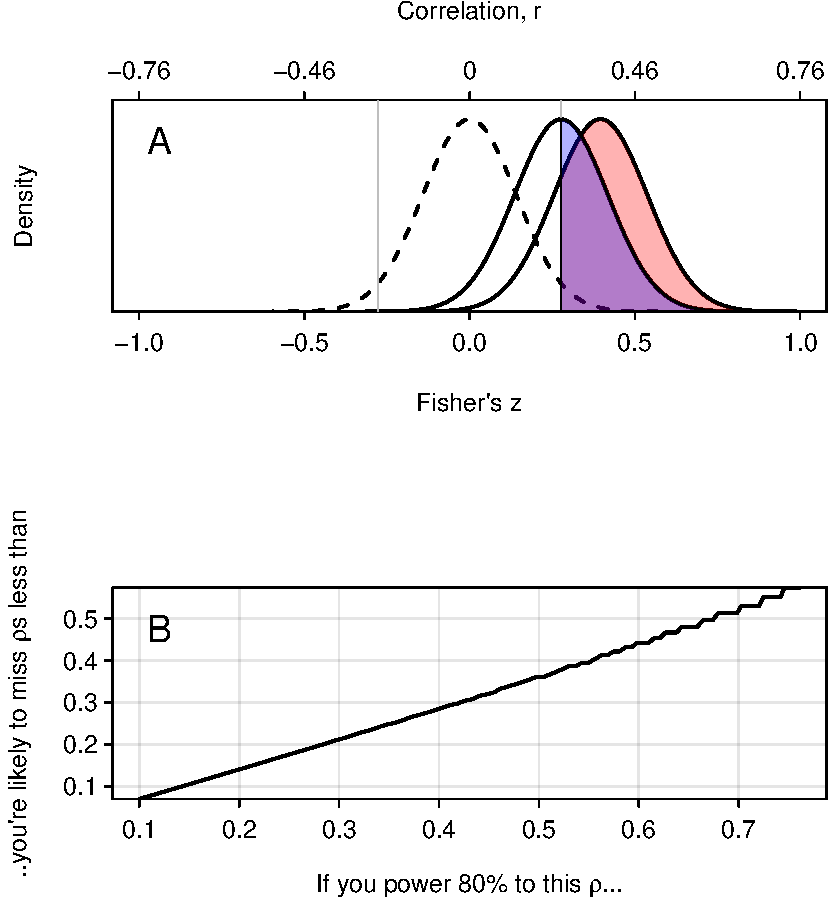
\includegraphics[width=\maxwidth]{figure/powfail-1} \caption{A: The effect size that yields 0.8 power is not far from the critical value. Thus, effect sizes less than about 70\% the size of the chosen effect size will be missed more than half the time. B: For every effect size chosen for 0.8 power, the corresponding effect size that will be missed half the time.}\label{fig:powfail1}
\end{figure}

Extending the fire alarm analogy, powering a study based on a previous result is like buying a smoke alarm sensitive enough to detect only the raging fires that make the evening news. It is likely, however, that such an alarm would fail to wake you if there were a moderately-sized fire in your home. One might attempt to calibrate the alarm by making it more sensitive to smoke (i.e. increase $\alpha$), but in the process one would make the alarm sound often in the presence of no smoke. Such an alarm would fail to serve its purpose. No one would trust such a fire alarm, and yet such alarms are analogous to vast numbers of hypothesis tests in the literature.

{\bf Misconception 4: Sample size choice should be based on what the effect is believed to be.}
Another common misconception, related to Misconception~3, is that sample size choice should be driven by a guess at what the effect size might be. This guess can be based on previous findings, but it can also be based on theoretical ideas. However, although one might {\em believe} an effect is large --- for any reason at all --- psychological theories are not specified precisely enough that they imply specific effect sizes. Importantly: knowledge that the effect is moderate almost never contradicts whatever theoretical viewpoint led one to believe that the effect was large. It is not one's beliefs about the most plausible value for an effect that should primarily drive sample size choice, but rather the desire to detect effects of meaningful sizes, or rule out other effect sizes that would falsify a theoretical prediction. 

The broad point here is that the power curve depends only on the properties of the test and chosen design, and the effect size used to power the design should be based not on what one believes or what someone has found in the past, but rather by the effect sizes one would like to detect (barring resource constraints, etc). Belief and previous results need not enter into the question at all, except to the extent that they inform one's sense of what an interesting effect size is.

Combined with publication bias (Sterling, 1959; see also Lakens, 2015) and flexible analysis methods (Gelman and Loken, 2014), we believe that these fallacies explain psychology's current problems with power. Most studies have low power, and hence statistical tests cannot differentiate even large effects from noise. Publication bias leads to large published effects by necessity, because at the small sample sizes common in the literature these are the only ones that are statistically significant. Researchers power to these large effect sizes, perpetuating the problem and creating a noise-laden literature. The consequence is that the literature is not a friend to theoretical progress, but rather its mortal enemy. 

\nocite{Sterling:1959,Gelman:Loken:2014,Lakens:2015}

\subsection{Moderators and cumulative science}
Although we have couched much of the discussion above in terms of the RP:P, the problem of low power does applies to all attempts to compare studies. Consider that the ability to build theory is based on the presumption that similarities and differences between studies can be assessed. Cumulative science requires building a body of evidence across many studies. If studies in experimental psychology are not sufficiently powered so that we can detect a difference from a similarly-sized close replication, they are not sufficiently powered to detect differences between conceptual replications, or two studies testing different theories, either. 

Some researchers have suggested that non-significant replications are caused by unknown moderators, the ``moderator hypothesis''. Of course, it is plausible that differences between studies may cause differences in results. However, the insight that true differences between original and replication studies cannot be detected with small samples has implications for the testability of the moderator hypothesis. Imagine that a team --- say, the original experimenters --- decided to assess the possibility that a particular moderator affected the results of an earlier experiment experiment with a small sample size. They design an experiment that is exquisitely controlled, differing only in the desired way from the original experiment, and they collect a large sample of participants, just to be safe. Our analysis shows that even this ideal approach is doomed to fail, because when the original sample size is small, even large differences between the original and replication study cannot be detected with high probability. Under these conditions --- which prevail in the psychological literature --- to argue for moderators is to interpret noise. 

What applies to replications also applies to non-replications as well. If one cannot argue that the results of two experiments are different, given the sample sizes typical in the statistical literature, cumulative science seems beyond reach. In fact, many discussions of both replications and variations on similar designs rest on a common statistical fallacy: asserting the difference between two effect sizes on the basis that one is significant and the other not. \citep{Gelman:Stern:2006}. An example makes this fallacy obvious: two effects based on the same sample size might yield $p$~values of $p=0.049$ and $p=0.051$ and thus differ in their significance, yet have nearly identical effect sizes. 

The Gelman and Stern fallacy was accepted when many of the RP:P replications failed to achieve significance: the original was significant, but the replication was not, so the replication ``failed.'' It is implicit, too, when a researcher makes a slight modification to a design and finds a significant effect where there was none before, then argues that the design change must have been responsible for the ``effect.'' It is also implicit when a reviewer requests that an author explain why they failed to find a significant effect where a previous study found one. In each scenario, small sample sizes across the literature mean that interpreting differences across studies --- like arguing for moderators to explain unsuccessful replications --- is likely to be interpreting noise.

\subsection{The problem of under-specified theory}

In 1964, Platt stated that whenever someone proposes a scientific explanation or theory, we should ask 'The Question': What would \textit{dis}prove your hypothesis? Our current analysis shows that unless a researcher specifies which effect sizes are too small to be considered support for the hypothesized effect, theories and explanations are not falsifiable. Consider the fact that many theories in psychology are supported merely by a significant effect in a particular direction. If the proponents of a psychological theory propose neither a minimum effect size consistent with their theory, nor a maximum difference from their original finding that would cause them to question it, then it is not clear what could disprove their hypothesis. This is perhaps the greatest problem that faces psychological science, and one that has received almost no attention in recent discussions about better research practices.

\nocite{Platt:1964}

Some researchers have argued that replication studies should aim to show equivalence using a very narrow equivalence bound (e.g., excluding true effects smaller than $d$ -0.05 or larger than 0.05, Maxwell, Lau, and Howard, 2015). The idea is that such small effect sizes are never support for a theory. This proposal implies an asymmetry: researchers who want to falsify a prediction need to collect thousands of observations, while a researchers who propose a theory can do so with a tiny sample size. Furthermore, in practice researchers mostly make directional predictions, and thus any effect reliably different from 0 can be claimed as support for a theory, even if this effect is smaller than d = 0.05. Claiming that any effect reliably different from zero supports your theory is not a falsifiable prediction, because in the extreme case, there are not enough people on earth to falsify it. Instead, we believe authors should make specific, falsifiable, predictions. This is the main way for theories to get money in the bank, so to speak (Meehl, 1990). 

\nocite{Meehl:1990,Maxwell:etal:2015}

One way to make more specific predictions is for psychology to move towards a specification of a smallest effect consistent with one's theoretical position. Considering the lack of such a specification alongside the small sample sizes,  much of psychology is {\em de facto} unfalsifiable. In drug research, deviations smaller than 20\% are deemed too small to matter. Simonsohn (2015) proposes to make the threshold dependent upon the observed sample size in the original study, by setting the smallest effect size of interest to the effect size the original study had 33\% power to observe. We now provide our own recommendations for powering future novel studies.

\nocite{Simonsohn:2015}

\section{Recommendations for powering future studies}

As shown above, the sample size of the original study imposes a limit on what is learned by a replication attempt. Although this limit is bad when replicating previous studies, it does reveal a way of thinking about powering studies in the future. We suggest that researchers power their studies so that a similarly-sized replication has a high probability of detecting a specified difference from the study, if that difference exists. Suppose we regarded two studies as being different --- and hence, not replications of one another --- if the true difference between the two is .1 Fisher's $z$ units. Further suppose we run 50 participants. Then the power of a similarly-sized experiment to detect a deviation of .1 at $\alpha=0.05$ is a mere .11. Figure~\ref{fig:reppower3} shows the power to detect various true differences as a function of sample size, assuming equal sample sizes in the original and replication experiments. In order to obtain 80\% power to detect a true difference of .1, we would require about 1,600 participants. For a similarly-sized replication to have 80\% power to detect a true difference of .3 would require about 175 participants. For comparison, the median sample size in the RP:P original studies was 54, which provides 80\% power to detect only deviations greater than .54 Fisher's $z$ units.


\begin{figure}
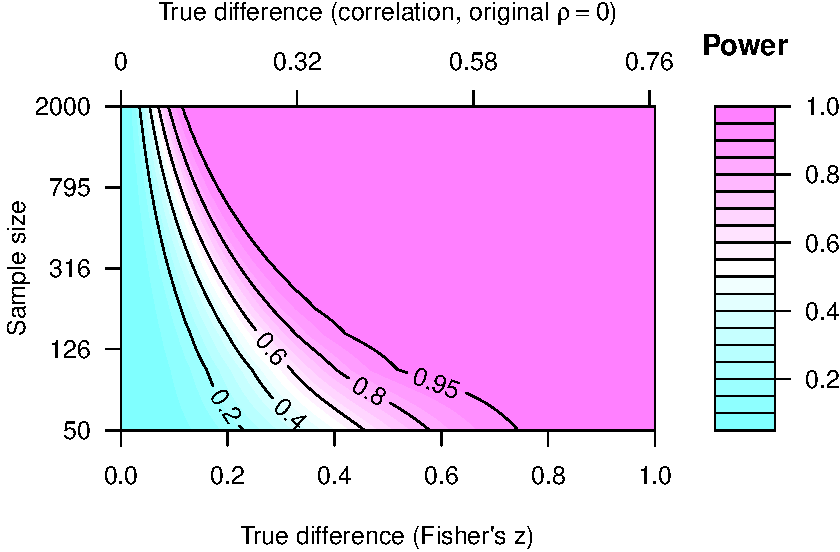
\includegraphics[width=\maxwidth]{figure/reppower3-1} \caption[Choosing a sample size for an original study such that a similarly-sized study has high power to find a true deviation of a given size from your results]{Choosing a sample size for an original study such that a similarly-sized study has high power to find a true deviation of a given size from your results.}\label{fig:reppower3}
\end{figure}

In general, the difference between two independent random quantities with the same variance will be twice that of either quantity. Therefore, if one powers their studies so that a future replication has a high power of detecting a difference between studies of $\delta$ units, one will need twice as many participants than if powering to detect a difference of $\delta$ from 0. This is the cost of a higher-resolution literature more amenable to cumulative science.

The approach to power we suggest here has several advantages. First, the difference between true effect sizes is related to the desired resolution of the results in the literature, and not a difficult-to-stipulate effect size. There is a close relationship between the approach we suggest here and the approach of aiming for narrow confidence intervals. In addition, the question of whether to power to a one-sided or two-sided hypothesis also disappears. One-sided hypotheses will still be possible, of course; they just would not be the primary concern when choosing a sample size.

More importantly, when we power to detect differences, we should explicitly treat every study as part of a larger scientific fabric instead of instead of seeing one study as an isolated attempt to answer a single question. In our view the current culture of individually wrapped, single-serving science must give way to a culture of comparison, integration, and sharing. The logic of much of experimental psychology involves making small changes in experimental conditions and attempting to understand any differences observed between the studies. The only way that experimental psychology can be cumulative, however, is if potential differences between studies can actually be detected. The typical approaches to power --- either not considering it, or powering studies based on previous findings --- leads to dramatically underpowered, unfalsifiable inferences, and a literature that cannot sustain the needs of cumulative science. 


\section{What about prediction intervals?}

Patil, Peng, and Leek (2016; henceforth PPL) have recently defined a replication as ``successful'' when the 95\% prediction interval for the effect size estimate of the replication study --- computed around the results of the original study --- includes the actual point estimate from the replication. In contrast to our analysis of the RP:P above, PPL apply prediction intervals to the same 73 studies we analyzed above\footnote{We made use of the analysis code they publicly released, available at \url{https://github.com/jtleek/replication_paper}.} and suggested, on the basis of their analysis, that there is reason for ``guarded optimism'' about the reliability of the psychological literature. We review their analysis here and show why it is not a meaningful approach to evaluating the success of replication studies.

\nocite{Patil:etal:2016,OpenScienceCollaboration:2015}

Typical confidence intervals (CIs) are constructed to have a fixed, long-run probability of containing the true value of a parameter; a prediction interval (PI), in contrast, is constructed to have a fixed, long-run probability of containing a future data point drawn from a population with the same parameter. Constructing the PI requires the original study's effect size, $r_{orig}$, the original study's sample size, $n_{orig}$, and the sample size of the replication, $n_{rep}$. 

According to PPL, a study is said to have replicated if the observed effect size of the replication is contained within the PI. The attraction of the PI approach is that it takes into account the uncertainty in the original study and the sampling error in the replication. They note that of the 92 replication attempts they examine, 69 (75\%) yielded effect sizes that fall within the 95\% PI of the original study. PPL claim that this number is reason for ``guarded optimism'', and implicitly contrast this with ``extreme'' media coverage reporting that 36\% of the replication studies failed to be statistically significant.

We first note that we omitted 19 of the 92 (21\%) studies PPL analyzed, due to the fact they they should not have been included. The correlations were based on effect sizes with multiple degrees of freedom in the numerator and hence the sampling distribution assumed by PPL was not correct. Of the remaining 73 replications, 51 (70\%) yielded effect sizes that fall within the original study's 95\% PI. We will use this number throughout, rather than PPL's 75\%.

There are a number of reasons why the analysis approach based solely on PIs should not, in fact, lead to optimism about the results of the RP:P.

{\bf The confidence coefficient is arbitrary.} PPL focus on the fact that that 70\% of the 95\% PIs contain the replication effect size. PPL do not justify the use of a 95\% confidence coefficient, and this choice seems to be based solely on convention. Figure~\ref{fig:conf.coef} shows the ``replication success'' rate as a function of the confidence coefficient for coefficients from 50\% to 99\%. If PPL would have used 99\% prediction intervals, an even more impressive total of 89\% of PI's would contain the replication effect sizes. On the other hand, only 29\% of the 50\% intervals contained the replication effect size, which worse. Interestingly, about only 34\% of the replication results were within one prediction standard error of the original result. This is just under the 36\% reported in the media and described as ``extreme'' by PPL. 

Which confidence coefficient best reflects how many replication studies ``successfully'' replicated the original finding? The prediction standard error, with its 34\% ``success rate,'' has {\em at least} as good a claim as the 95\% PI. The use of a 95\% prediction interval is based solely on convention and is not a well-motivated measure of replication success. This is true both when effect size estimates in original studies are very inaccurate, as when they are extremely accurate, where trivial differences can be outside the PI. 

\begin{figure}
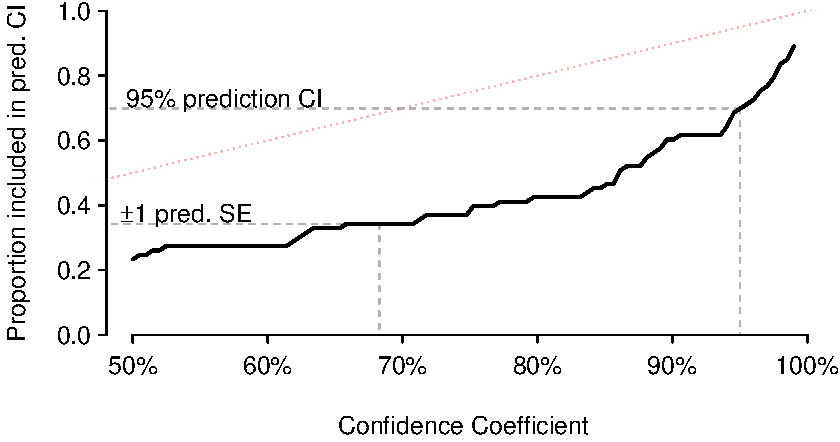
\includegraphics[width=\maxwidth]{figure/conf_coef-1} \caption[Proportion of replication attempts within the prediction intervals as a function of confidence coefficient]{Proportion of replication attempts within the prediction intervals as a function of confidence coefficient.}\label{fig:conf.coef}
\end{figure}

{\bf The ``good'' success rate is arbitrary.} A second weakness of the prediction interval perspective is that it is difficult to interpret the ``success rate''. Is 70\% high or low? Consider framing the results in terms of the failures, rather than the `successes'': we would expect only 5\% of the replications to be outside the prediction intervals, but instead we find 30\%, a six-fold increase from what we would expect. Or suppose we represent the results in terms of odds instead of probabilities: we expected 19 successes for every one ``failure'', yet we observed only 2.3 successes for every failure. 

We can also add context to the 70\% by asking what would happen if the original studies had been plagued by various kinds of problems. Suppose, for instance, that instead of reporting the observed effect size, all original authors had reported an effect size of exactly zero. In this case, the success rate actually {\em improves} to 81\%. If, on the other hand, we randomly permute the original studies' effect sizes so that there is no relationship between the original and replication effect sizes, the ``success rate'' only drops to 54\% on average. The 70\% success rate is therefore closer to what one expects with randomly permuted effect sizes than the nominal 95\%. Given these examples, a 70\% success rate sounds less impressive.\footnote{One might object that both of these demonstrations work because the relative to the width of the PIs, the replications are close to 0 and fairly similar. That is precisely is the point: the PIs are so wide that they are an insensitive way of assessing replication success.}

{\bf Interval reasoning is dichotomous.} Consider a replication study in which the effect size is very close to the original, yet just outside the prediction interval. This can occur when both the original and replication sample sizes are very large, as in fact they were in study pair {\em c} in Table~\ref{tab:studies} (see also Figure~\ref{fig:resid1}). In contrast, large deviations from the original can be missed solely because the sample sizes are small. A reliance on the PI treats all pairs for which the PI includes the replication as the same, and all in which the PI excludes the replication as the same. 

The logic of asserting a replication based on inclusion within a PI is also backward. To see this, note that confidence intervals, including PIs, can be thought of as inversions of significance tests: a $100(1-\alpha)$ CI contains all hypotheses that would not be rejected by a particular two-sided $\alpha$ level test. Of what significance test is PI an inversion? As it turns out, the PI is the inversion of the test of no difference that we deployed in the previous section, using the test statistic $z_d$. This equivalence is reasonable: if the prediction made on the basis of the results of the original study fails, then we infer that the two studies have different underlying effect sizes. 

The equivalence between the PI and the significance test is more than a statistical curiosity. Since the statement ``the $100(1-\alpha)$\% PI contains the replication effect size'' is equivalent to ``the null hypothesis that $\rho_{orig}=\rho_{rep}$ is not rejected at level $\alpha$'', this means that PPL's criterion for a successful replication --- and the related inference that ``data collected from the replication are drawn from the same distribution as the data from the original experiment'' (PPL, p. 542) --- is based on a non-significant test of no difference. The use of prediction intervals has encouraged PPL to fall into a classic fallacy in significance testing: asserting the null hypothesis is true on the basis of a non-significant result.

We do not believe that the RP:P provides reasons for ``guarded optimism''. In fact, in showing that typical sample sizes yield practically unfalsifiable results, the RP:P has revealed deep problems with the experimental psychological literature.

\section{Conclusion}

As psychology begins to realize it needs well-designed studies with sufficient power to draw informative inferences from data, the question is: what do we want to learn? Here, we have argued that an important inference we want to draw in cumulative science is whether an observed effect is similar or different from other studies in the literature. The combination of under-powered studies and misconceptions about how to design well-powered studies has resulted in a literature that cannot support the needs of a cumulative science: very large differences between studies cannot be detected with high probability, and sample sizes are often so small that even high-powered replications cannot call original studies into question. Hypothesized moderators are of no help, for the same reason: at typical sample sizes, the power to detect a difference due to a moderator in ideally-controlled experiments would be very low.

By offering pairs of studies with similar sample sizes and methods, the Replicability Project: Psychology results have enabled us to bring the problem into focus. Moving forward, we recommend psychological researchers power their studies to give others the chance to refute them in a replication, or build off of them by exploring potential moderators. This requires powering studies to {\em differences} between hypothetical studies, rather than merely to find an effect of interest.

In our view, psychological researchers must begin to think less about how to {\em obtain} an effect and more about to to {\em test} an effect. A focus on the former has given rise to flexible analysis methods \citep{Gelman:Loken:2014} and a literature filled with ``significant'' effects and tidy narratives. A focus on the latter, however, requires us to address a version Platt's (1964) question: {\em What would call this result into doubt?} Current low-resolution designs and vague theory mean that much of psychology is not practically falsifiable. We hope that the current generation succeeds where previous ones failed: psychological science where power and precision are treated with the respect they deserve.

%\clearpage
\printbibliography


\clearpage
\appendix

\section{Fisher's $z$ transformation for correlations}


\begin{figure}
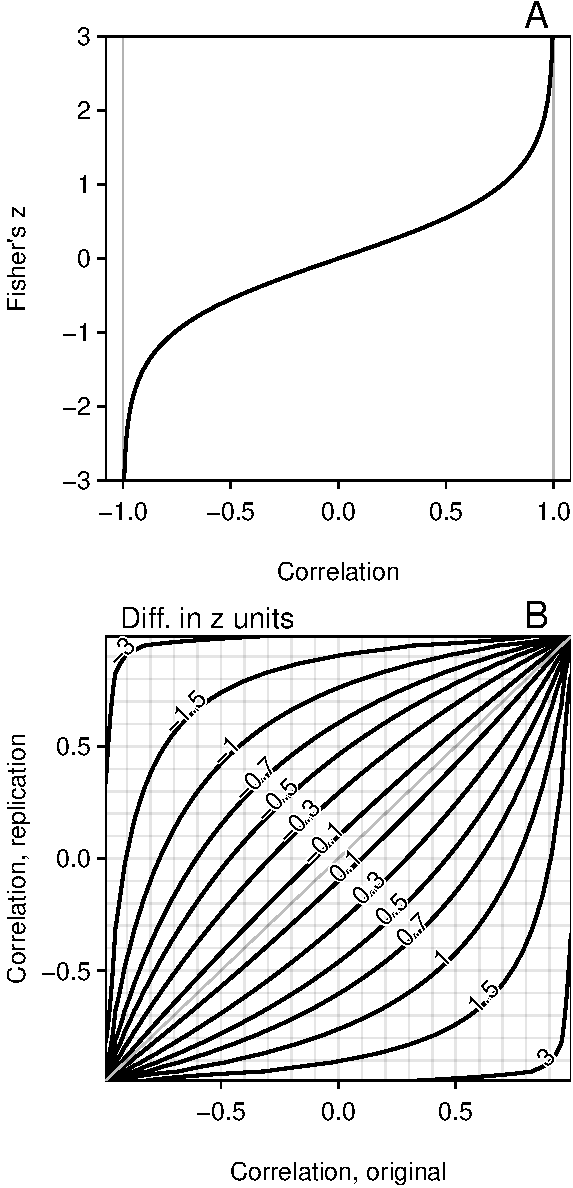
\includegraphics[width=\maxwidth]{figure/zexp-1} \caption{Top: Fisher's $z$ transformation takes the bounded correlation and maps it to the unbounded $z$ units. Bottom: Contour showing differences in Fisher's $z$ units as a function of the original and replication correlations.}\label{fig:zexp1}
\end{figure}

Because correlations are bounded between -1 and 1, the variance of a correlation differs depending on whether the correlation is near 0 (high variance) or near -1 or 1 (low variance). A convenient way of treating correlations is to transform them from $[-1,1]$ to $[-\infty,\infty]$ using Fisher's $z$ transformation, shown in Figure~\ref{fig:zexp1}. We denote this transformation as $z(r)=\mbox{arctanh}(r)$. The associated inverse transformation, from $z$ to $r$, is $r(z)=\mbox{tanh}(z)$. The same transformation is used for the true correlation, $\rho$.

Fisher's $z$ transformation is convenient: if two random variables have a bivariate normal distribution\footnote{We use the correlation estimates computed by the OSC and Fisher's $z$ transformation as assumed by Patil, Peng, and Leek (2016). The broad points we make here do not depend on these particular assumptions; alternative tests making fewer assumptions will tend to have less power, not more, and so our results represent a best-case scenario.}, then $z(r)$ will be normally distributed with a mean that depends only on $\rho$, the true correlation coefficient, and variance that depends only on the number of sample points, $n$:
\[
Z = z(r) \stackrel{.}{\sim} \mbox{Normal}\left(z\left(\rho\right), 1/\sqrt{n-3} \right). 
\]

\nocite{Patil:etal:2016}

If the sampling distribution of $Z$ is normal, then the sampling distribution of the difference between two independent $z$-transformed correlations also has a normal sampling distribution, a fact which makes building significance tests and confidence intervals easier. We make use of this fact throughout the manuscript.

\end{document}
